\documentclass{article}
\usepackage{amsmath, amsthm, amsfonts, bm, graphicx, xcolor, soul, mathtools, parskip}

\title{CSC401 Lecture 3 Summary}
\author{Mir Shafayat Ahmed}

\begin{document}
    \pagecolor[HTML]{FFFFCC}
    \maketitle
    \section{Entity Relationship Diagram}
        Why?\\
        When it comes to handling data, process oriented system doesn't work. With that approach data duplication occurs. And this destroys data integrity. Editing one of them will need others to be edited as well. A nightmare.
        \paragraph{}
        Data is stable, it is unlikely to change. But processes are subject to more frequent changes. So, if processes are updated, chaos ensues. So we keep Processes and Data Separated.
        \paragraph{}
        So we want to create a model where we show how different database entities relate.\\
        A student may have id, name, address etc. These are stable. But the process of updating them may change, hence, separation is preferred.
        \paragraph{}
        In many systems, hybrid approaches are taken where Relational Databases and other types of Databases are mixed. It all depends on our system.

        \subsection{Entities}
            Entity is that data object on which we want to maintain data on.\\
            A course entity may have many characteristics, ID, Name, Description etc.
            \subsubsection{Strong Entity Type}
                An entity that exists independent of other entity types. A student is a strong entity type.\\
                Denoted by Rectangle.
            \subsubsection{Weak Entity Type}
                The existence of these entities depends on other Strong Entity Types. A section of a course is an example.\\
                Denoted by REctangle within Rectangle.
            \subsubsection{Associative Entity Type}
                When an Entity Type is used to associate one entity type to another entity type.\\
                Denoted by Rounded Rectangle.

            \subsubsection{What should Entities Be}
                They can be an object that can have many instances.\\
                They will have multiple attributes.\\
                We shouldn't make them from  input and output od the database.\\
                We dont model entities if the entity does not contribute to data in our database. Such as a guardian of a student. THey may be allowed to see a report of the student but the guardian does not need to be modelled.
            \subsubsection{Naming Enitity Type}
                \begin{itemize}
                    \item Must be a \emph{singular noun}.
                    \item Name should be specific to the organization.
                    \item Short names or abbreviation.
                    \item 
                \end{itemize}

        \subsection{Attributes}
            Required Attributes and Optional Attributes exist.
            \subsubsection{Simple vs. Composite Attributes}
                An address can be broken down into smaller components. If so, then it will be a composite attribute.\\
                But we can treat it as a whole, a simple/atomic attribute. Similar to Name. 
            \subsubsection{Single-valued vs. Multivalued}
                We should keep in mind if a single instance can have multiple valued attributes such as Phone number.\\
                But for example, they cannot have multiple ids.
            \subsubsection{Stored vs. Derived}
                An attribute that can be calculated or derived from another attribute is a derived attribute.
            \begin{figure*}[h]
                \centerline{
                    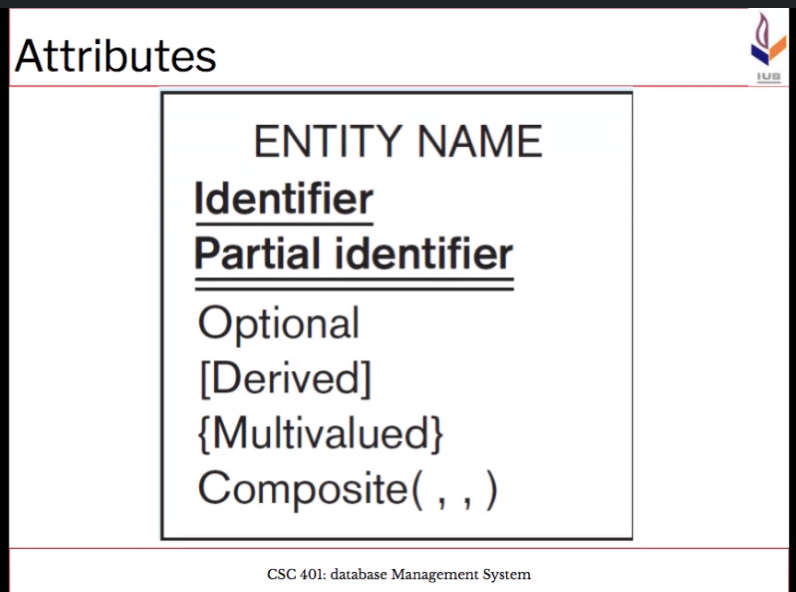
\includegraphics[scale=0.2]{Entity rules.png}
                }
            \end{figure*}
        \subsection{Identifiers or Key Attribute}
            An attribute or combination of attributes (Composite), that uniquely identifies an entity.\\
            Cannot be NULL.
        
        \subsection{Relationship Lines discussed}
            \begin{figure*}[h]
                \centerline{
                    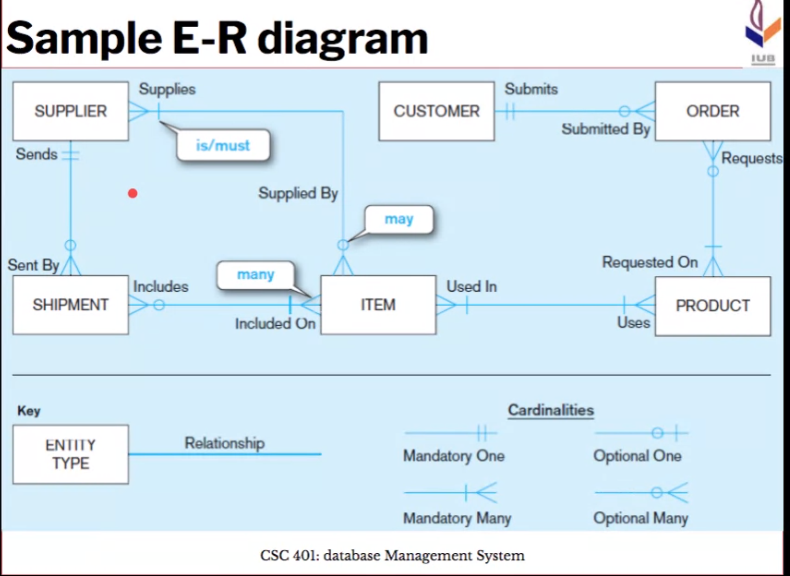
\includegraphics[scale=0.4]{Sample ERD.png}
                }
            \end{figure*}


\end{document}